\chapter{Methodology}
\label{Methodology}

In this section, we introduce the methodology for our proposed approaches for the task of human pose estimation using the point cloud. As we reviewed in Chapter~\ref{Related work}, the key issue of any model which uses point clouds as input data, it's a huge spatial variation of the data. Point clouds much diverse compared to 2D images in terms of location and rotation. Capsule networks show promising results on 2D data \parencite{sabour_dynamic_2017}, and such models handle better spatial invariance compared to regular NN models.

The chapter consists of two main sections. In Section~\ref{Data-preparation} we cover the preprocessing for the input data and ground truths and methods of adding artificial noise to the input data. 

In Section~\ref{Network architecture} we cover the network's architecture and algorithms for performing network training.


\section{Data preparation}
\label{Data-preparation}
In this section, we cover the main preprocessing steps for datasets. Preprocessing consists of:
\begin{enumerate}
  \item human extraction;
  \begin{enumerate}
    \item threshold filtering;
    \item clusterization \& human cluster selection;
  \end{enumerate}
  \item point cloud normalization;
  \item adding noise to data (optional).
\end{enumerate}

In the first step, we remove the most obvious points which don't represent human posture. In the second step, we perform clustering and segmentation to extract "human" clusters. The third step is optional and is used in Section~\ref{s:experiment-noise} where we measure the performance of different models with various levels of noise. 

All steps of the preprocessing pipelines are shown in Figure~\ref{img:example-of-all-parts}: threshold filtering, clusterization, and segmentation.

\begin{figure}[htbp]
    % \centerline{
    \hspace*{-1cm}                                                           
        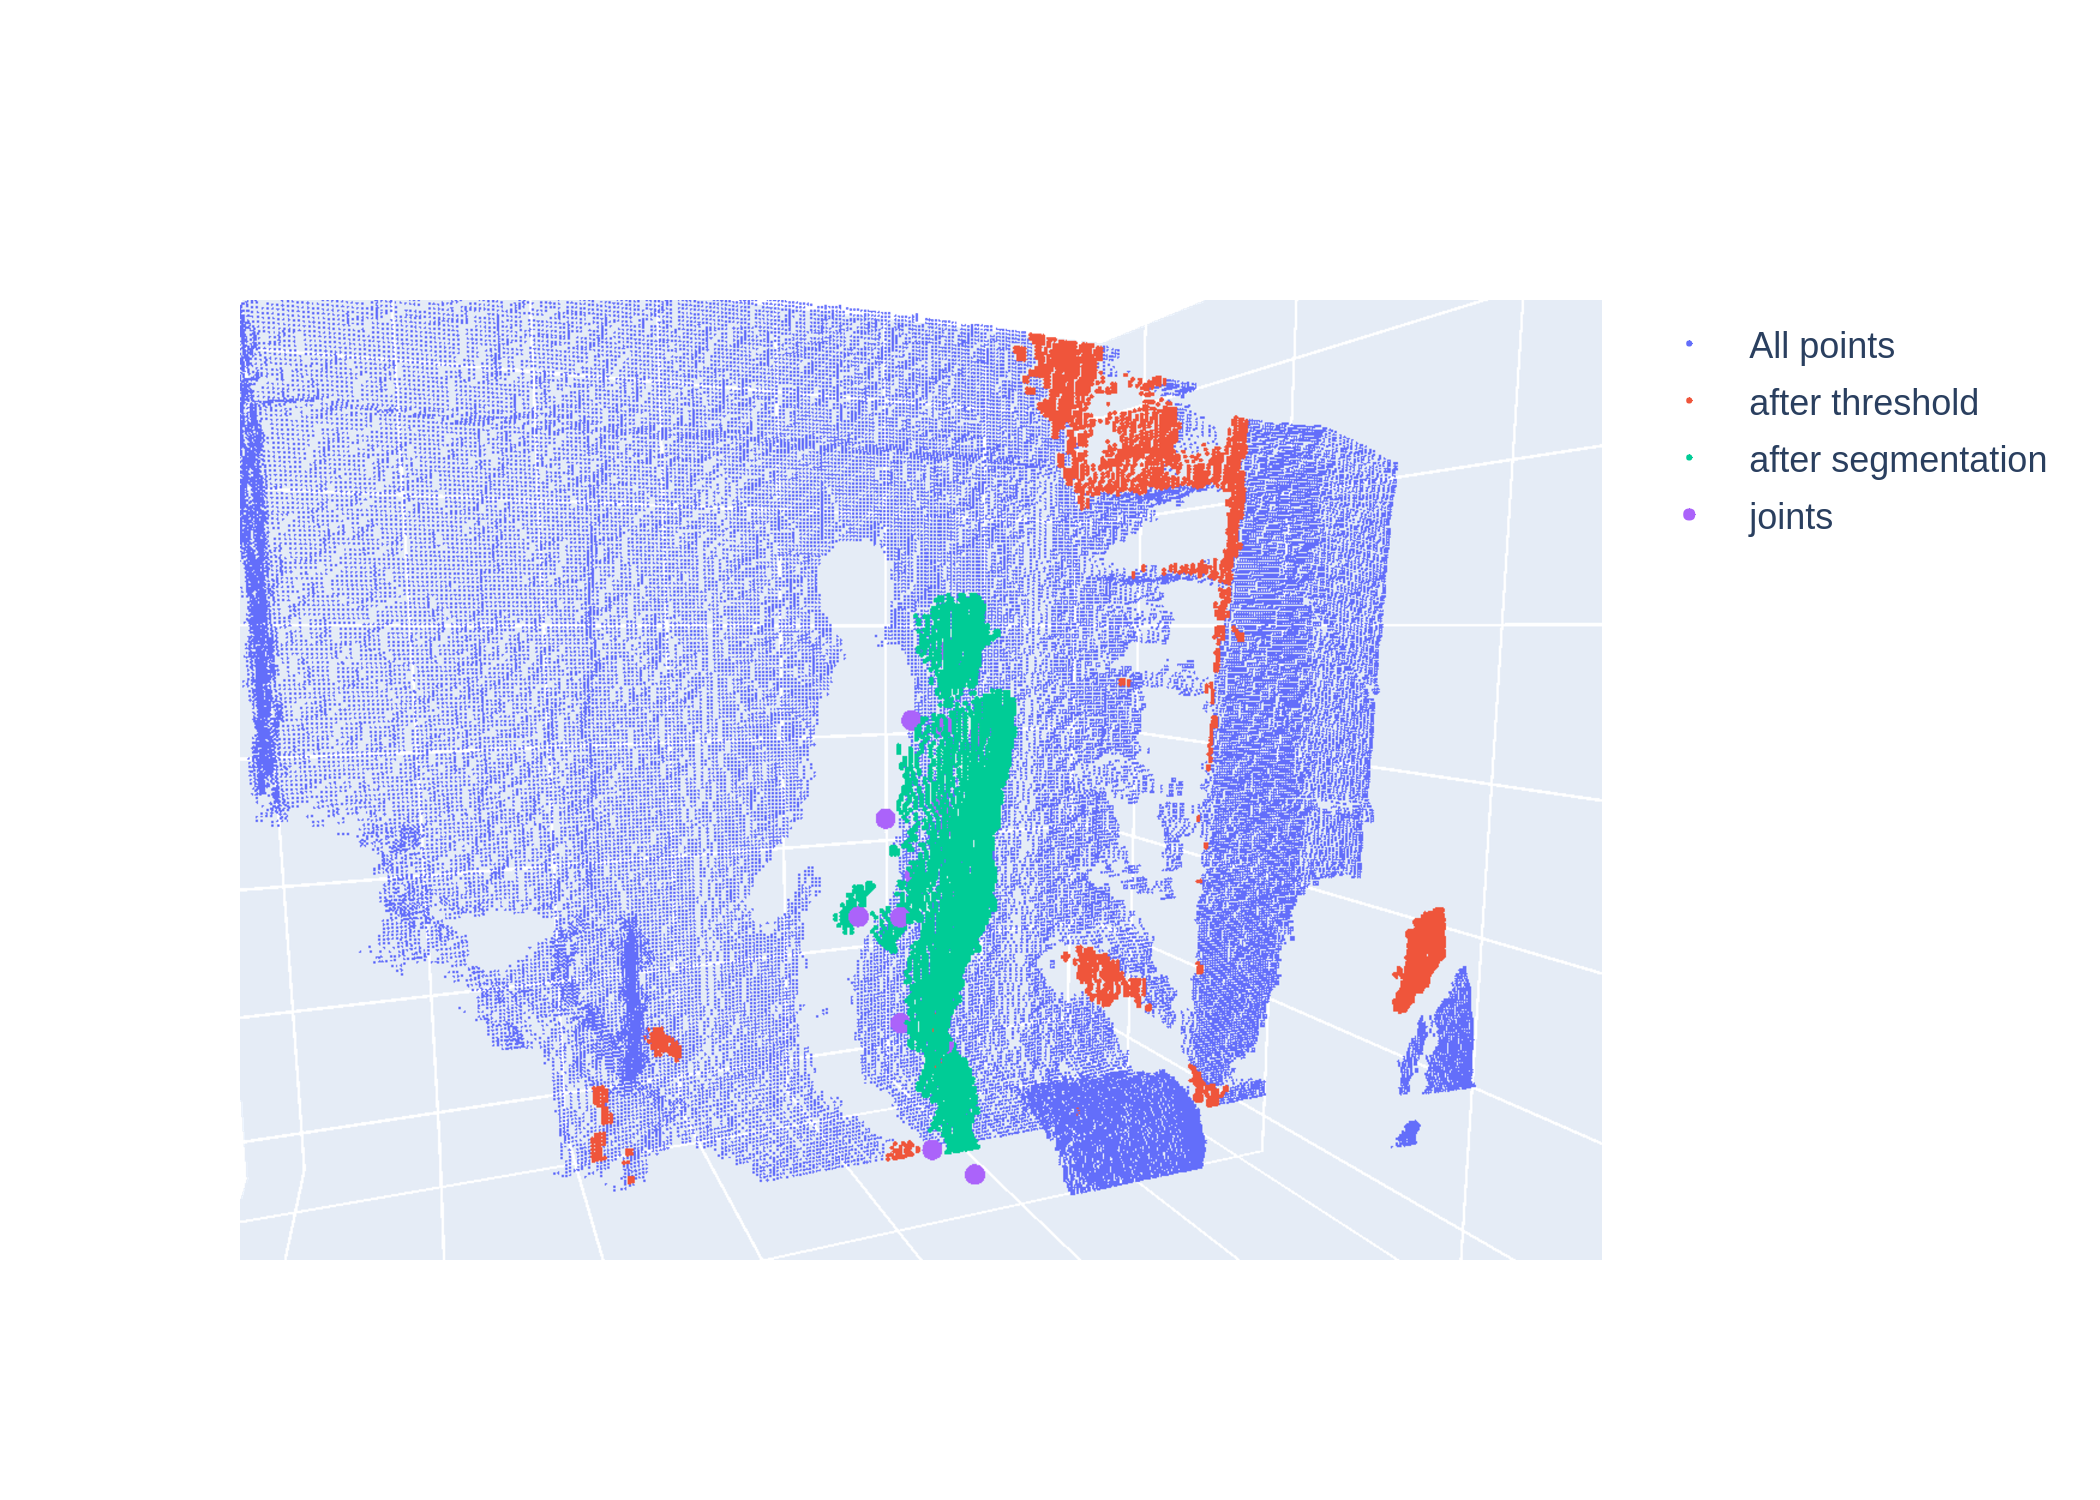
\includegraphics[trim=0 200 450 200,clip,scale=0.25]{Figures/example-all-parts.png}
    % }
    \caption{Example of preprocessing stages. \textbf{Blue} - points filtered by threshold. \textbf{Red} - points removed by human segmentation. \textbf{Green} - extracted human point cloud. \textbf{Purple} - key human joints}
    \label{img:example-of-all-parts}
\end{figure}

\subsection{Human extraction}
To start working with point cloud for human pose estimation we need to extract human points out of the overall point cloud. As we can see from Figure~\ref{img:example-of-raw-data}, the raw point cloud contains not only a human point cloud but also other objects which are located in the room, such as walls, cupboards, and other objects. These obstacles will not only harm the model's performance but will also greatly slow the model's training and inference due to the excess number of points.

\begin{figure}[htbp]
    \centerline{
        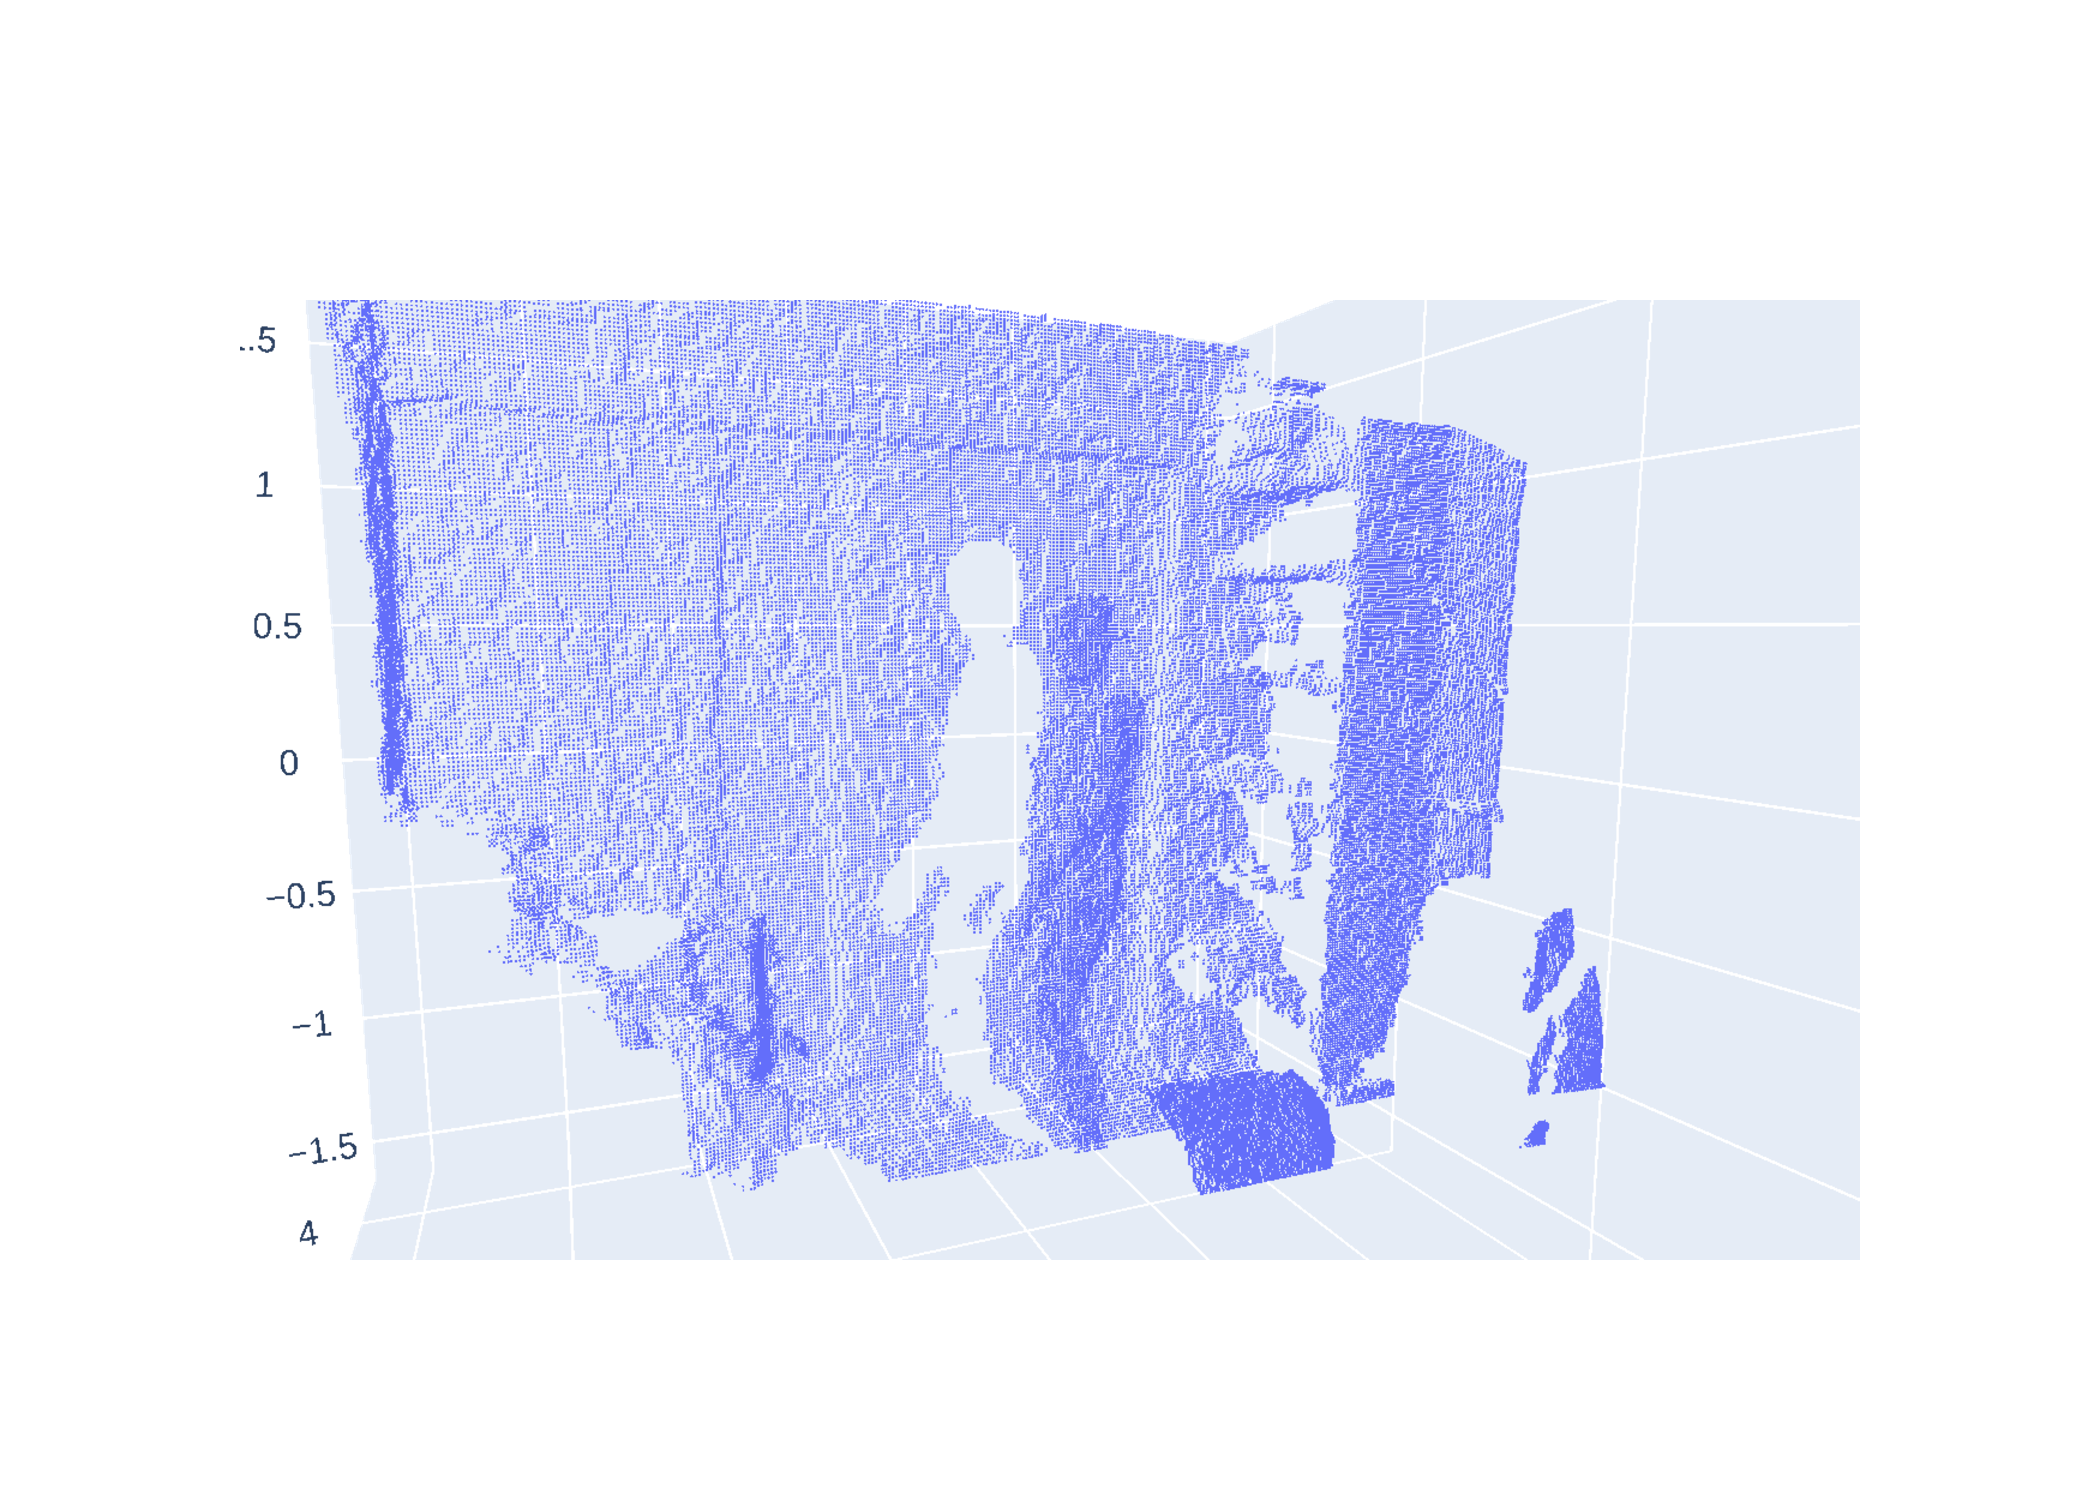
\includegraphics[trim=370 200 400 200,clip,scale=.25]{Figures/example-of-raw-data.png}
    }
    \caption{Example of raw data from ITOP dataset (front view)}
    \label{img:example-of-raw-data}
\end{figure}

\subsubsection{Threshold filtering}
\label{s:threshold-filtering}
Threshold filtering is the first step in preprocessing pipeline. The aim of this step is to filter out the most obvious points which don't belong to the human posture.
After manual checks we came up to such parameters side view dataset:  

\begin{equation}
    \begin{aligned}
        x_{min} &= -1   &x_{max} &= 1 \\
        y_{min} &= -1.4 &y_{max} &= 2 \\
        z_{min} &= -1.5 &z_{max} &= 3.5
    \end{aligned}
\label{eqn:threshold-values-side}
\end{equation}

and for top view dataset:

\begin{equation}
    \begin{aligned}
        x_{min} &= -0.91   &x_{max} &= 0.85 \\
        y_{min} &= -0.63 &y_{max} &= 0.57 \\
        z_{min} &= 0 &z_{max} &= 2.6
    \end{aligned}
\label{eqn:threshold-values-top}
\end{equation}

Formula~\ref{eqn:threshold-values-side} and \ref{eqn:threshold-values-top} set min-max distance values from camera view. The camera sensor is considered as center - $(0, 0, 0)$. In this way, $x$ coordinate represents left-right direction from the camera center, $y$ - top-bottom, and $z$ - the depth. \\
An example of a threshold filtered point cloud could be seen in Figure~\ref{img:after-threshold-filtering}.

\begin{figure}[htbp]
    \centerline{
            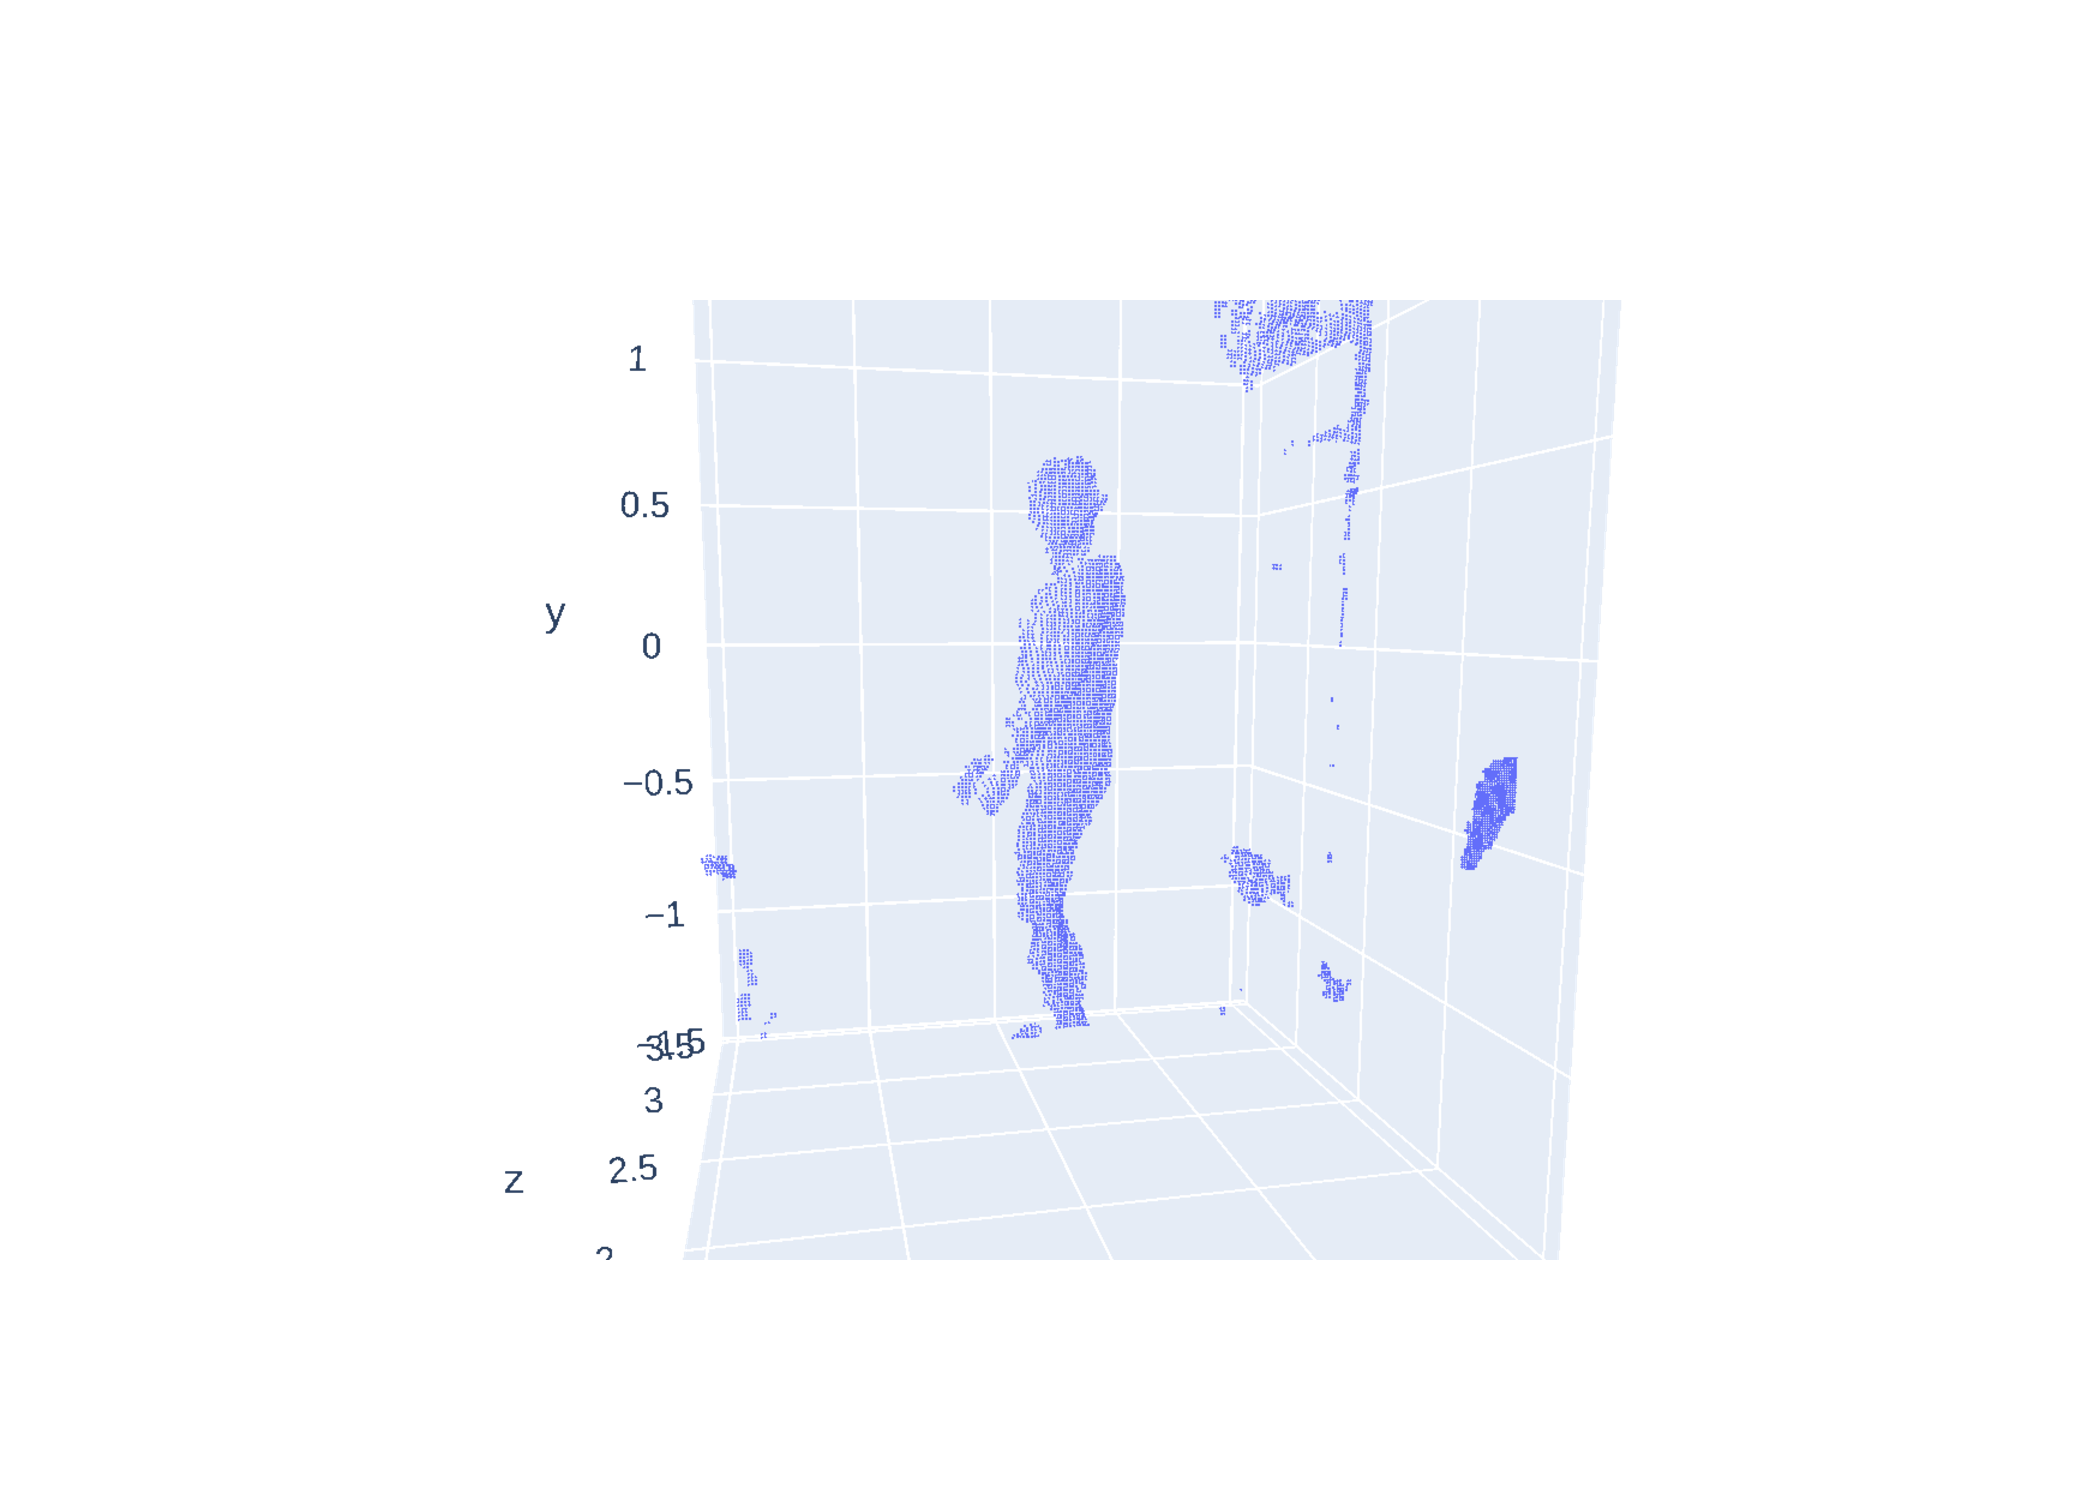
\includegraphics[trim=750 200 700 200,clip,scale=.35]{Figures/example-after-threshold.png}
    }
    \caption{Example of point cloud after applying of threshold filter}
    \label{img:after-threshold-filtering}
\end{figure}

Since thresholds were manually selected it's crucial to validate that all human points clouds fit these boundaries. In our case, we run checks on resulting point clouds after the segmentation step which will be described later. By this check, we confirmed that at the end of our extraction pipeline each example in the dataset contains exactly one big cluster (number of points $>2000$). This check doesn't guarantee that our method works well on each example, but it's enough to say with high probability that it works on the vast majority of cases. However, it's worth stressing that this step in our pipeline could be improved in future work.

\subsubsection{Clusterization}
Clusterization \& extraction are the next steps in preprocessing pipeline. In this step, we cluster the point cloud from the threshold filtering step (Subsection~\ref{s:threshold-filtering}) and extract the human cluster. For clusterization step we propose the nearest-neighbour search algorithm \parencite{noauthor_nearest_2021} with kd-tree data-structure, using FLANN \footnote{Fast Library for Approximate Nearest Neighbor}.

The aim of the clusterization is to separate human clusters and small noisy clusters from the point cloud. As we can see from the Algorithm~\ref{alg:clusterization}, for each point in the initial point cloud $P$ we try to put it to some cluster based on the distance (radius - $r$) to that cluster. If the distance is less than the radius to each cluster then this point creates a new cluster. At the end of clusterization, we get a set of clusters $C$. \\
Since the human cluster always the biggest, at the end of clusterization we take the argmax and get human cluster $C_{human}$.

In the previous paragraph, we made an assumption that human is the biggest cluster out of all clusters. Although the assumption holds for the ITOP dataset it doesn't guarantee the same performance for other datasets. Thus, this step in preprocessing pipeline could be improved in future work.

In Figure~\ref{img:after-clustering} we can see the point cloud before clusterization, after, and the resulting human cluster (the biggest cluster).

\begin{figure}[hbt!]
    \centerline{
            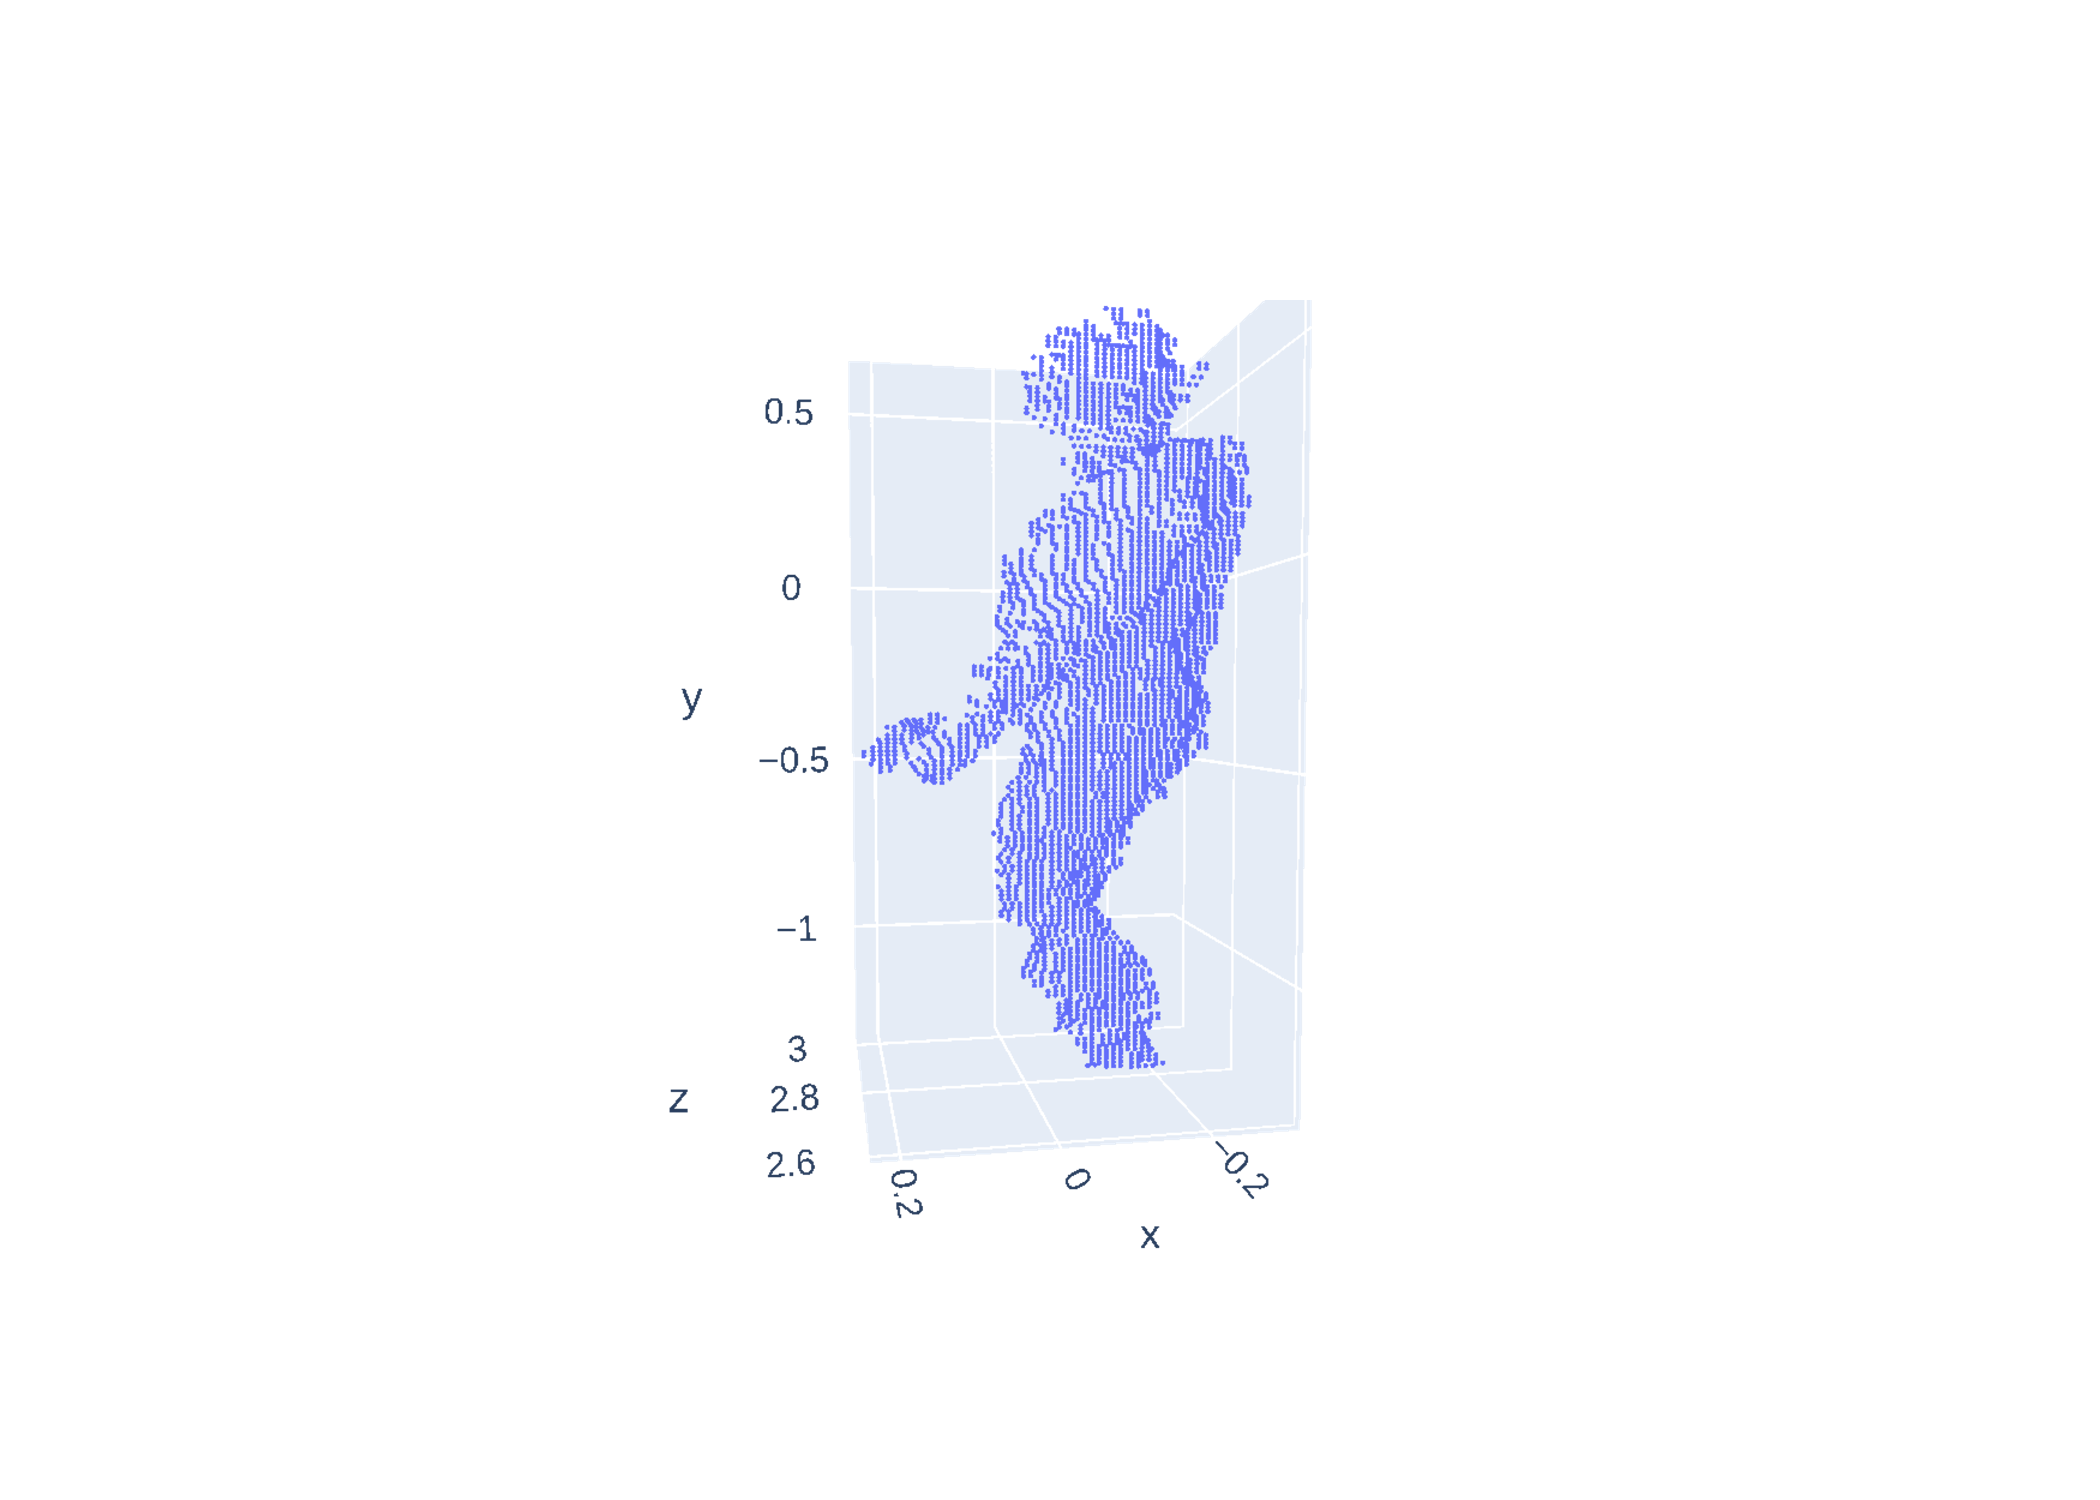
\includegraphics[trim=850 400 700 200,clip,scale=.3]{Figures/example-after-segmentation.png}
    }
    \caption{Example of point cloud after applying human extraction}
    \label{img:after-clustering}
\end{figure}

\begin{algorithm}[H]
\label{alg:clusterization}
\SetAlgoLined
\KwResult{human point cloud cluster - $C_{human}$}
 create a Kd-tree representation for the input point cloud dataset $P$ \;
 set up an empty list of clusters $C$, and a queue of the points that need to be checked $Q$ \;
\For{\texttt{every point} $p_i \in P$} {
    add $p_i$ to the current queue $Q$ \;
    \For{\texttt{every point} $p_i \in Q$}{
        search for the set $P^k_i$ of point neighbors of $p_i$ in a sphere with radius $r < d_{th}$ \;
        for every neighbor $p^k_i \in P^k_i$, check if the point has already been processed, and if not add it to $Q$\;
    }
    when the list of all points in $Q$ has been processed, add $Q$ to the list of clusters $C$, and reset $Q$ to an empty list \;
}
the algorithm terminates when all points $\boldsymbol{p}_i \in P$ have been processed and are now part of the list of point clusters $C$ \;
$C_{human} = \underset{ x \in C }{\arg\max}$

\caption{Point cloud clusterization and human extraction \parencite{noauthor_pcl_nodate}}
\end{algorithm}

\subsection{Point cloud normalization}

To allow the network to learn more quickly the optimal parameters for each point cloud we normalize the input data to a standard scale.

We use the classic normalization technique where we scale the data to have zero mean and unit variance. We calculate the mean and max values for each axis $X$, $Y$, and $Z$. Then we scale point cloud and ground truth key joints coordinates according to these values. (see Formula~\ref{eqn:normalization-points} and Formula~\ref{eqn:normalization-joints}).

\begin{equation}
    \begin{aligned}
        P_{normalized} = \frac{P - \textbf{mean}(P)}{\textbf{max}(P) - \textbf{min}(P)}
    \end{aligned}
\label{eqn:normalization-points}
\end{equation}
\begin{equation}
    \begin{aligned}
        J_{normalized} = \frac{J - \textbf{mean}(P)}{\textbf{max}(P) - \textbf{min}(P)}
    \end{aligned}
\label{eqn:normalization-joints}
\end{equation}

To calculate reconstruction and regression loss for the network we need to denormalize reconstructed point cloud, and regressed key joints coordinates. For denormalization, we use the same mean, max, and min values by which we normalized the data in the first place (see Formula~\ref{eqn:denormalize-points} and Formula~\ref{eqn:denormalize-joints}).

\begin{equation}
    \begin{aligned}
        \hat{P}_{\textbf{denormalized}} = \hat{P} \cdot (\textbf{max}(P) - \textbf{min}(P)) + \textbf{mean}(P)
    \end{aligned}
\label{eqn:denormalize-points}
\end{equation}

\begin{equation}
    \begin{aligned}
        \hat{J}_{\textbf{denormalized}} = \hat{J} \cdot (\textbf{max}(P) - \textbf{min}(P)) + \textbf{mean}(P)
    \end{aligned}
\label{eqn:denormalize-joints}
\end{equation}


\subsection{Adding noise to data}
\label{s:adding-noise-to-data}
Noise is the common thing in point cloud data. The origin of the noise could be environmental conditions such as dust, fog, and other particles in the air. Also, the noise appears due to the unperfectness of the lidar and other sensors creating point clouds.

In Experiment~\ref{s:experiment-noise} we investigate how models perform on data with different amounts of artificial noise. For that, we need to generate noise which could be similar to the real world. We propose to use two types of noise which are widely used \parencite{hermosilla_total_2019,lv_point_2020,rakotosaona_pointcleannet_2020}:
\begin{itemize}
  \item Gaussian noise;
  \item outlier noise.
\end{itemize}

\subsubsection{Gaussian noise}
The Gaussian noise adds noise to the initial points in the point cloud $P$. With probability of $p$ the Gaussian noise ($\sigma$, $\mu$) is added to the point $p \in P$. In this way, we simulate the unperfectness of the detecting device when the device makes measurements with some fraction of error. The generation process is described in Algorithm~\ref{alg:gaussian-noise}

\begin{algorithm}[H]
\label{alg:gaussian-noise}
\SetAlgoLined
\KwResult{human point cloud with Gaussian noise  - $\hat{P_{human}}$}
\For{\texttt{every point} $p_i \in P$} {
    \If{ \texttt{uniRand()} < $Prob_{noise}$ } {
        Set $p_x$ to $p_x$ + $Gaus(\sigma, \mu)$ \;
        Set $p_y$ to $p_y$ + $Gaus(\sigma, \mu)$ \;
        Set $p_z$ to $p_z$ + $Gaus(\sigma, \mu)$ \;
    }
}
\caption{Adding Gaussian noise to point cloud \parencite{uchida_tom-uchidaadd_noise_to_point_cloud_2021}}
\end{algorithm}

An example of applying the Gaussian noise to the point cloud could is shown in Figure~\ref{img:gaussian-noise}

\begin{figure}[htbp]
    \centerline{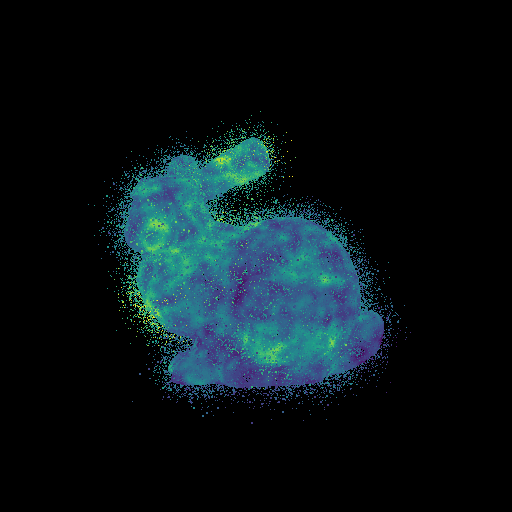
\includegraphics[scale=.6]{Figures/coords_gaussian.png}}
    \caption{Example of pllying the Gaussian noise to the point cloud \parencite{uchida_tom-uchidaadd_noise_to_point_cloud_2021}}
    \label{img:gaussian-noise}
\end{figure}

\subsubsection{Outlier noise}
The outlier noise adds new points to the initial point cloud $P$. The amount of outlier noise is defined by the fraction of the noise points compared to the initial number of human points. The noise point is taken from the uniform distribution $U(a, b)$. Where $a$ and $b$ are min-max values from the initial point cloud. In this way, outlier noise uniformly fills the bounding box of the initial point cloud.

An example of the addition of the outlier noise to the point cloud is shown in the Figure~\ref{img:outlier-noise}

\begin{figure}[htbp]
    \centerline{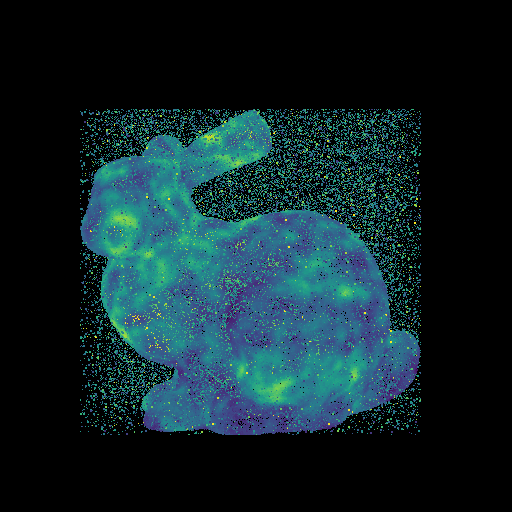
\includegraphics[scale=.6]{Figures/coords_outlier.png}}
    \caption{Example of addition the outlier noise to the point cloud \parencite{uchida_tom-uchidaadd_noise_to_point_cloud_2021}}
    \label{img:outlier-noise}
\end{figure}

\section{Network architecture}
\label{Network architecture}

In this section, we cover the network architecture for the task of human pose estimation, the loss functions, and the process of training.

We designed a network based on the work of \cite{wu_3d_2020} to estimate the human pose. In this work, we perform a one-stage training strategy compared to the previous two-sage approach. The aforementioned work performs two-stage training. The first stage consists of training an autoencoder part (based on capsules) of the network to recreate the input human point cloud. The second stage takes an autoencoder with frozen layers from the first stage and trains a regression part of the model which uses capsule outputs as input data. Such an approach requires two steps in the training pipeline and increases the number of hyperparameters to tune the network. In this work, we propose a one-stage training scheme which is described in Section~\ref{s:one-stage-network-training}.

\begin{figure}[htbp]
    \centerline{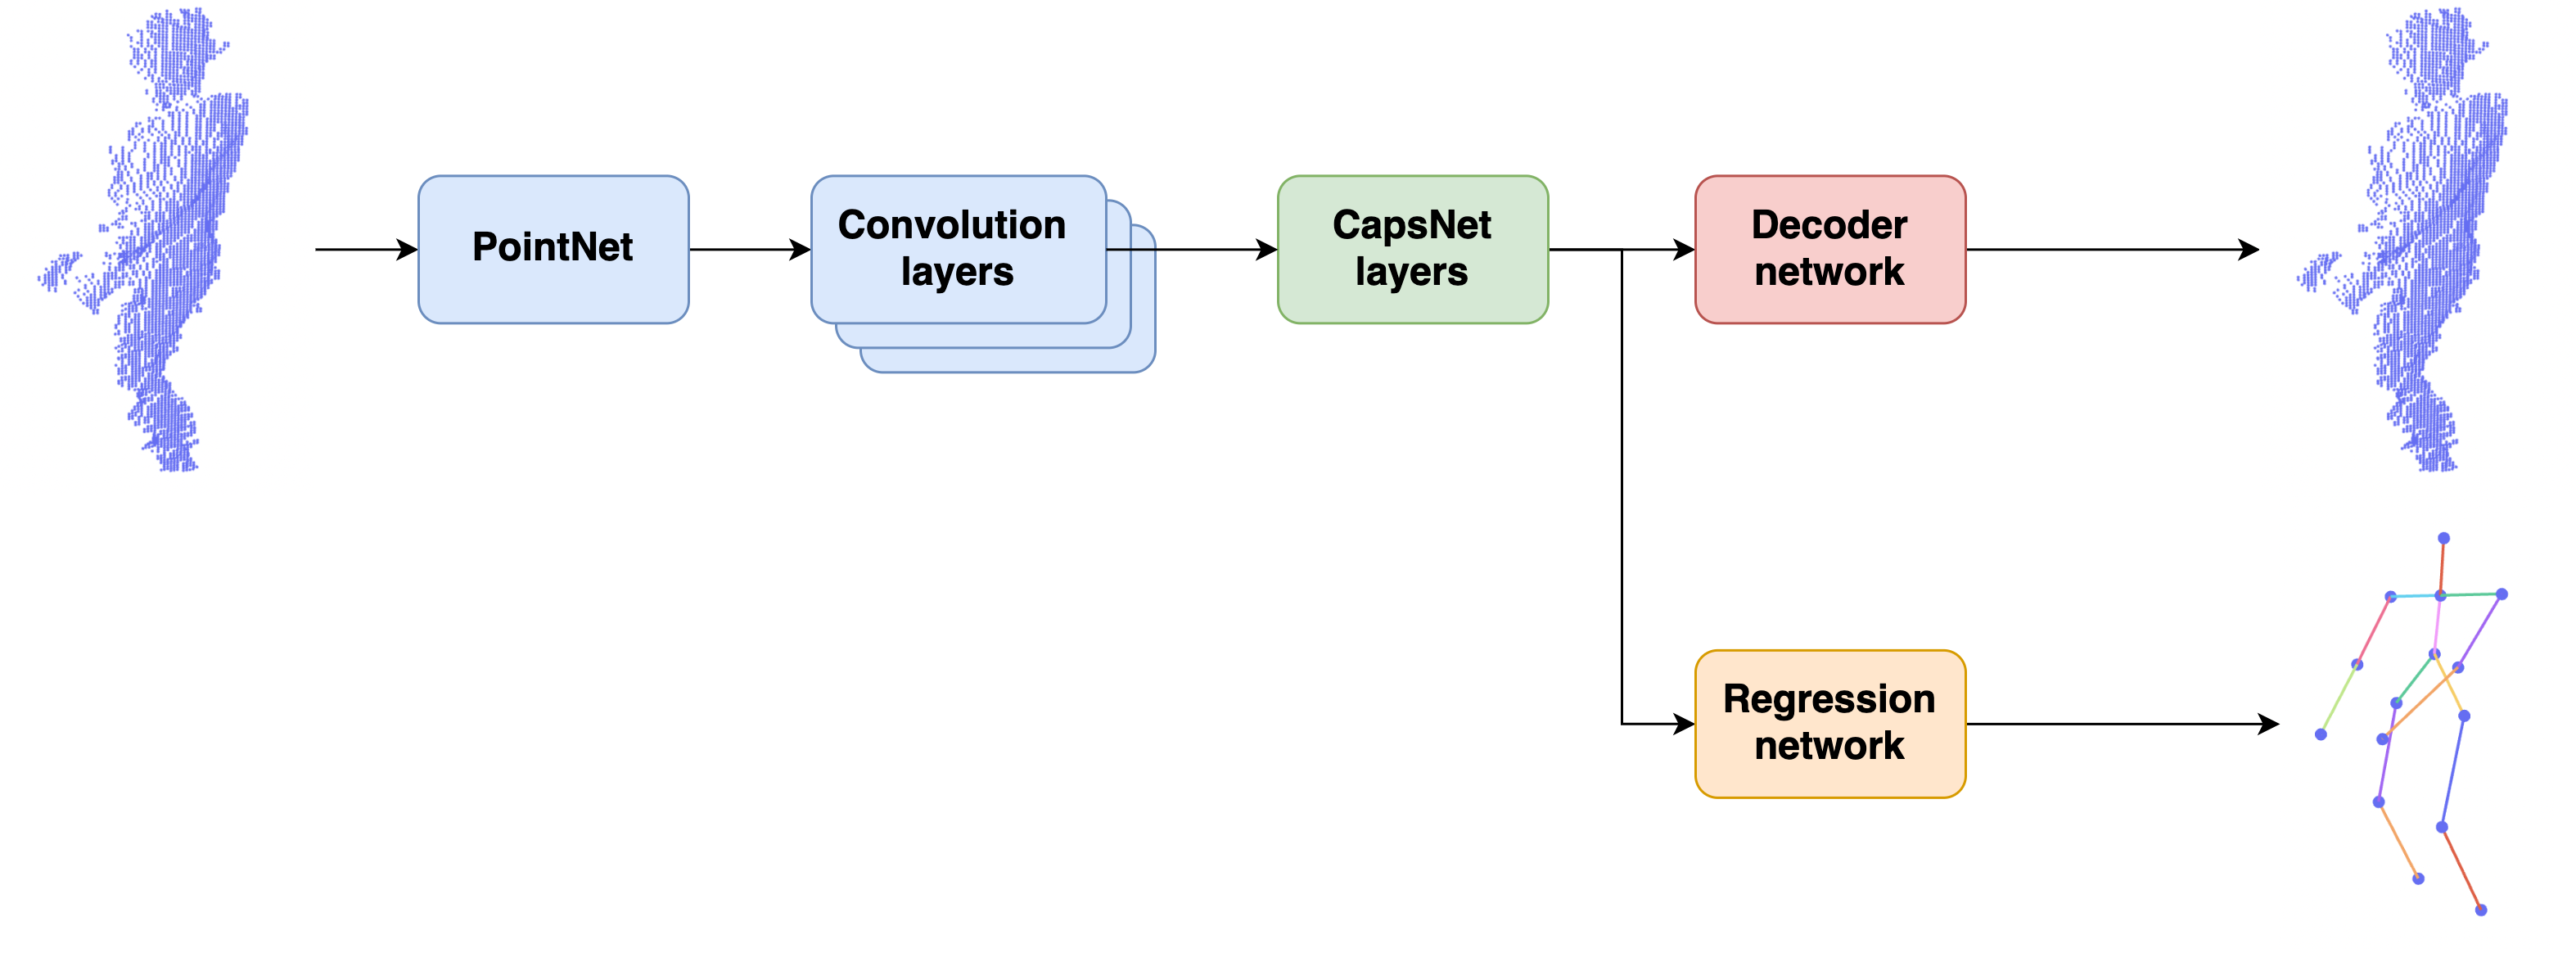
\includegraphics[scale=.125]{Figures/network architecture.png}}
    \caption{Network architecture}
    \label{img:network-architecture}
\end{figure}

\subsection{Loss aggregation}
In this work, we propose one-stage training based on loss aggregation. 
We will compare the results of the training with both a two-stage training scheme and a simple "loss sum" aggregation strategy in Section~\ref{s:one-stage-training}.
We use Chamfer distance as a loss function for encoder-decoder part. The Chamfer distance is defined as:

\begin{equation}
d_{C D}\left(P_{1}, P_{2}\right)=\sum_{x \in P_{1}} \min _{y \in P_{2}}\|x-y\|_{2}^{2}+\sum_{y \in P_{2}} \min _{x \in P_{1}}\|x-y\|_{2}^{2}
\label{eqn:chamfer-distance}
\end{equation}

Where $P_1 \in R^3$ and $P_2 \in R^3$ represent point clouds from the human point cloud and the point cloud recovered from latent capsules.

For the regression part of the network, we use classical MSE\footnote{mean squared error} loss.
The regression loss is defined as:
\begin{equation}
    \operatorname{Loss}_{E}(T, J)=\frac{1}{N} \sum_{i=1}^{N}\left(\left\|j_{i}-F\left(t_{i}\right)\right\|^{2}\right)+\lambda\|w\|^{2}
\label{eqn:regression-loss}
\end{equation}
Where $T$ is a feature vector from latent capsules. $J$ is the ground truth human joints. And $F$ is the regression network.

Since two losses have a different magnitude of values and at different points of time could differ in terms of "picking the low hanging fruit", we need aggregation to mitigate such issues.

The common approach of loss aggregation is usage of the weighted sum of losses \parencite{redmon_you_2016,cipolla_multi-task_2018,zhao_loss_2018} (e.g. $L = (af_1+bf_2)$ where $L$ is loss function, $a, b$ - loss weights, and $f_1, f_2$ - aggregated loss functions). These approaches struggles from increased huperparameter size since weights for losses should be chosen by hand.

We have selected an aggregation based on logarithms of losses' product. Such a decision is based on the assumption that our losses greater than $0$ and the magnitude is not drastic. The logarithm, in this case, mitigates the issue of vanishing gradient in the case when two losses approaching zero.

The result loss function is shown in Formula~\ref{eqn:aggregated-loss}.

\begin{equation}
    L = \log{(\operatorname{Loss}_{E}(T, J))} + \log{( d_{C D}\left(P_{1}, P_{2}\right))}
\label{eqn:aggregated-loss}
\end{equation}

The methodology of comparing different approaches is covered in \ref{s:one-stage-network-training}. The experiment comparison between one-stage training vs two-stage training is covered in \ref{s:one-stage-training}.

\section{One stage network training}
\label{s:one-stage-network-training}
In this section, we describe the method of training the model in one stage manner compared to two staged in \cite{wu_3d_2020}.

The work \cite{wu_3d_2020} proposes to split the training phase into two steps: the auto-encoder training phase and the regression training phase.

In the first phase regression network is frozen (Figure~\ref{img:network-architecture}) and PointNet, convolution layers, capsule layers, and decoder are trained. 

In the second phase, \cite{wu_3d_2020} propose taking the trained auto-encoder part from the previous step, freeze, and train only the regression part.

Our proposed solution is to train two forks of the network simultaneously. To achieve this we propose to aggregate two losses from each network's heads (decoder and regression). Doing this we expect to improve the performance of the network in terms of speed and accuracy.

The details of losses aggregation are covered in Section~\ref{s:how-noise-affects-models-performance}.

To verify the hypothesis that such an approach should improve the model's performance we will compare two cases: classical two-stage, and our proposed one stage. As a benchmark, we will use the ITOP dataset with the mAP metric described in Formula~\ref{eqn:dataset-metric-map}. The experiment results could be found in Section~\ref{s:one-stage-network-training}.
 

\section{How noise affects model's performance}
\label{s:how-noise-affects-models-performance}

In this section, we describe a pipeline of models' evaluation with noisy data. The noise generation technique is described in Section~\ref{s:adding-noise-to-data}.
We compare our model with SOTA model for the task of human pose estimation on ITOP \parencite{haque_towards_2016} dataset. Current SOTA is PoseNet \parencite{moon_v2v-posenet_2018} model.

The assumption we try to test is that a capsule-based network should perform better with noisy data due to the internal representation of the point cloud inside the network. The internal representation is held by latent capsules. In this way, the capsule-based network, due to its reconstruction part, should act like a denoiser which should help in the regression part of the task. The expected behavior of the model is shown in Figure~\ref{img:denoising}. Contrariwise, models which don't contain internal representation should perform worse on the same dataset.

\begin{figure}[htbp]
    \centerline{
            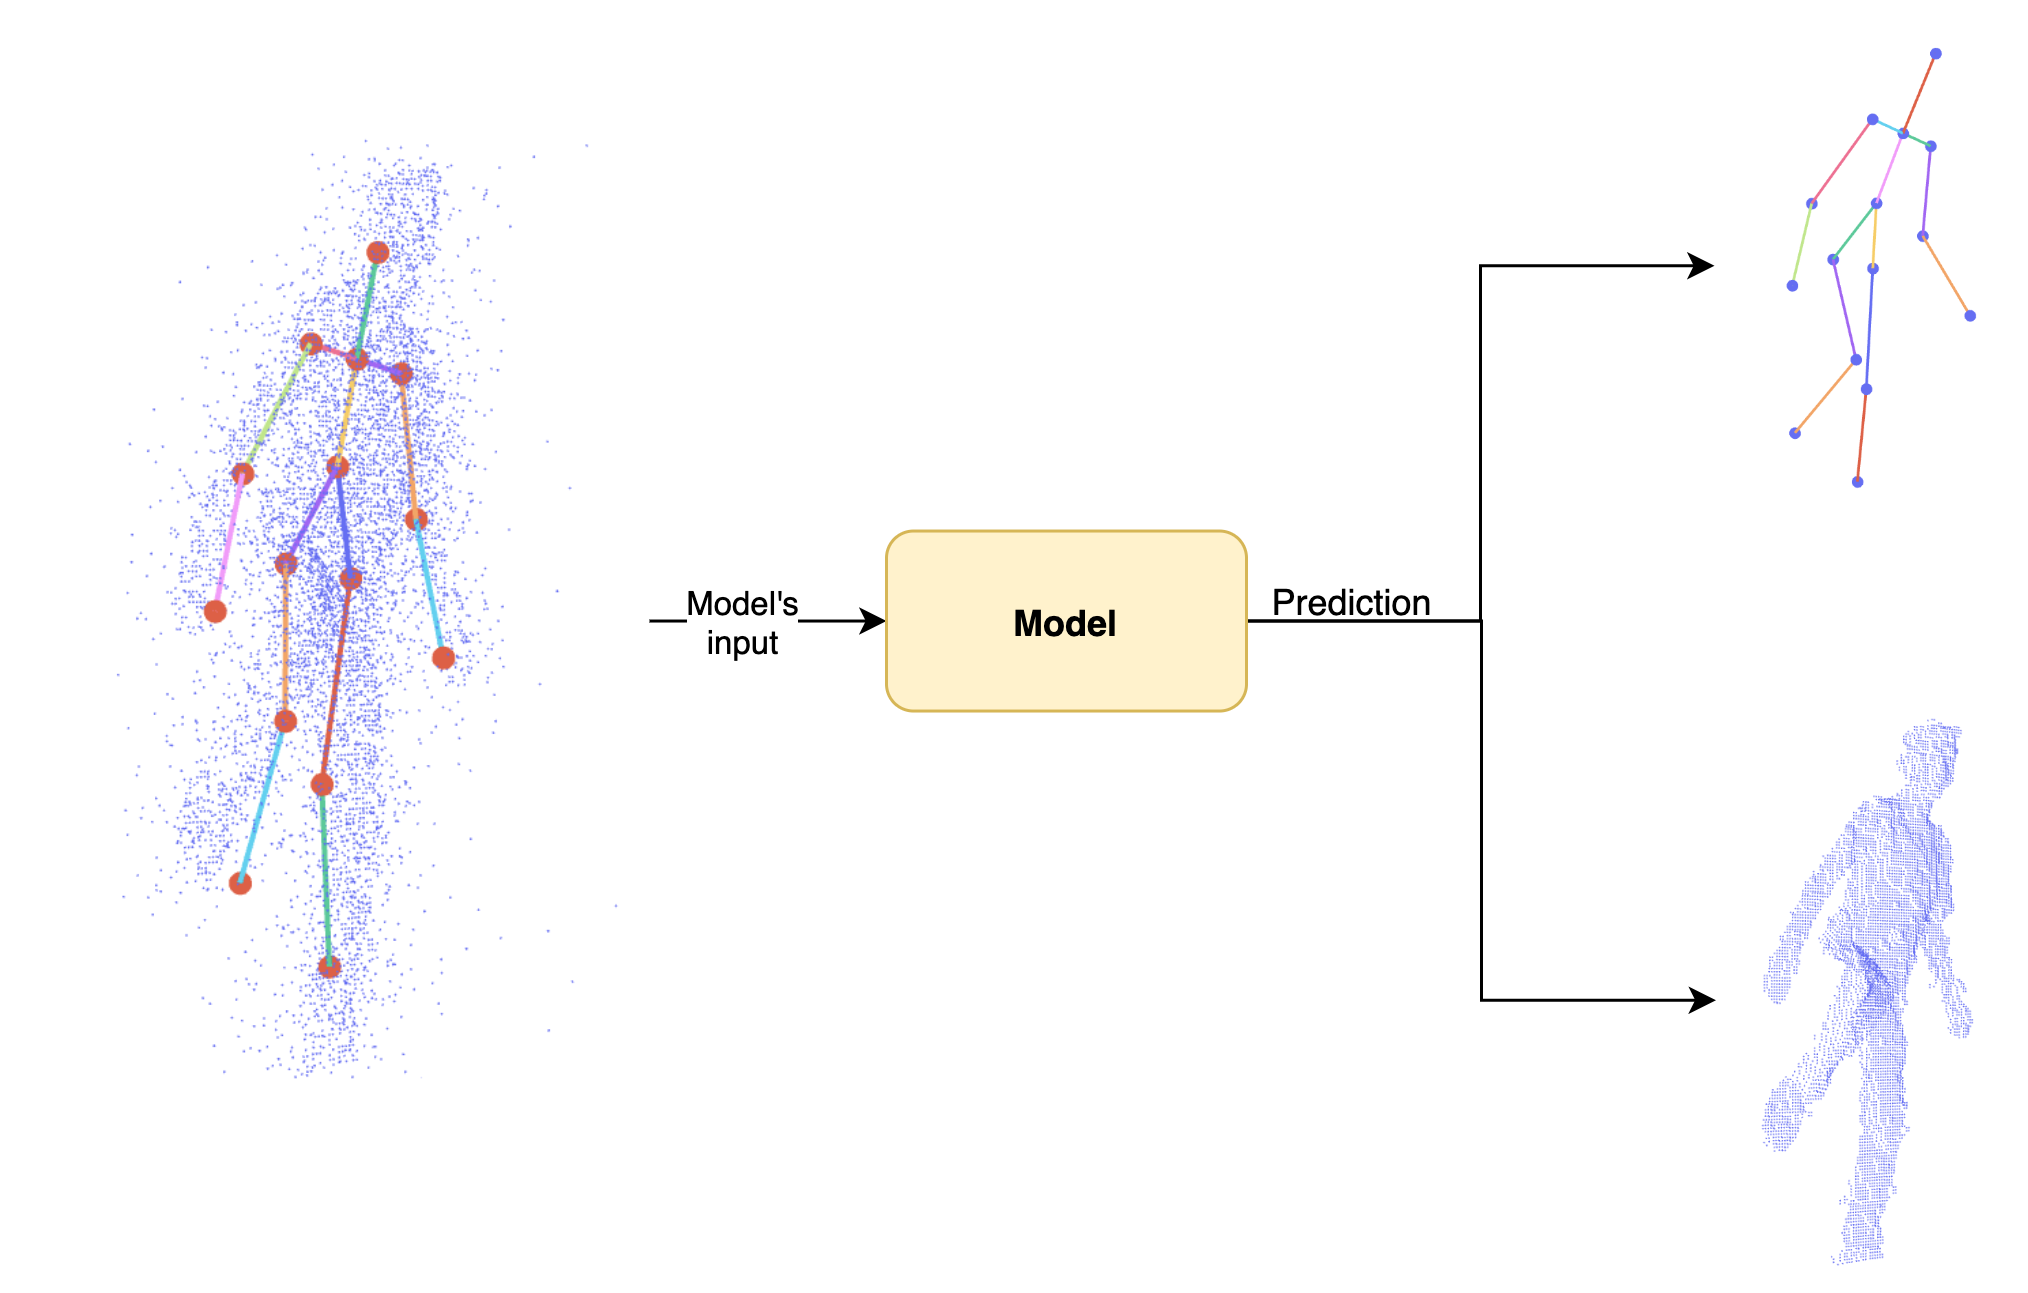
\includegraphics[scale=.2]{Figures/noise-model-scheme.png}}
    \caption{Capsule model trained on noiseless dataset expected to act like denoiser on noisy data}
    \label{img:denoising}
\end{figure}

To test the above assumption we use a capsule-based model which was trained on the dataset without noise and evaluate it on an evaluation set with a different amount of uniform and Gaussian noise. Also, we use the pre-trained PointNet model as a reference.
We will measure the absolute drop of mAP (described in Formula~\ref{eqn:dataset-metric-map}) with each increase of the noise amount.

\section{Influence of dataset size on model's performance}
\label{s:influence-of-dataset-size-on-models-performance}

In this section, we describe the pipeline of model evaluation for the experiment with a reduced training set.

In this part, we try to test the assumption that capsule-based models need less training data to perform equally on the evaluation set compared to non-capsule-based models. This assumption was proven for classification tasks on the MNIST dataset in \cite{sabour_dynamic_2017}, but wasn't reproduced on more complex data.

The capsule-based model due to its internal representation should faster come up with point cloud patterns compared to classical approaches. In this way, capsule-based models need less training data to perform equally on the evaluation dataset.

To test the above assumption we will train capsule-based model and SOTA model (PoseNet) with different fractions of training set till convergence. Then, we will evaluate the performance of both models on the evaluation set. We will measure the absolute drop of mAP (described in Formula~\ref{eqn:dataset-metric-map}) with each fraction of the training set.

The dataset reduction is done by removing unique people from the set. In the ITOP training dataset there are 16 unique people which result in $39,795$ point clouds.

We will use the model's performance on $100\%$ dataset (full train dataset) as reference values for both models. Then we will decrease the train dataset size to $15/16 \  - \ 93\%$, $12/16 \  -\  75\%$, and $8/16 \ - \ (50\%)$ from the overall size. The schematic visualization of dataset reduction is shown in Figure~\ref{img:dataset-split}.

\begin{figure}[htbp]
    \centerline{
            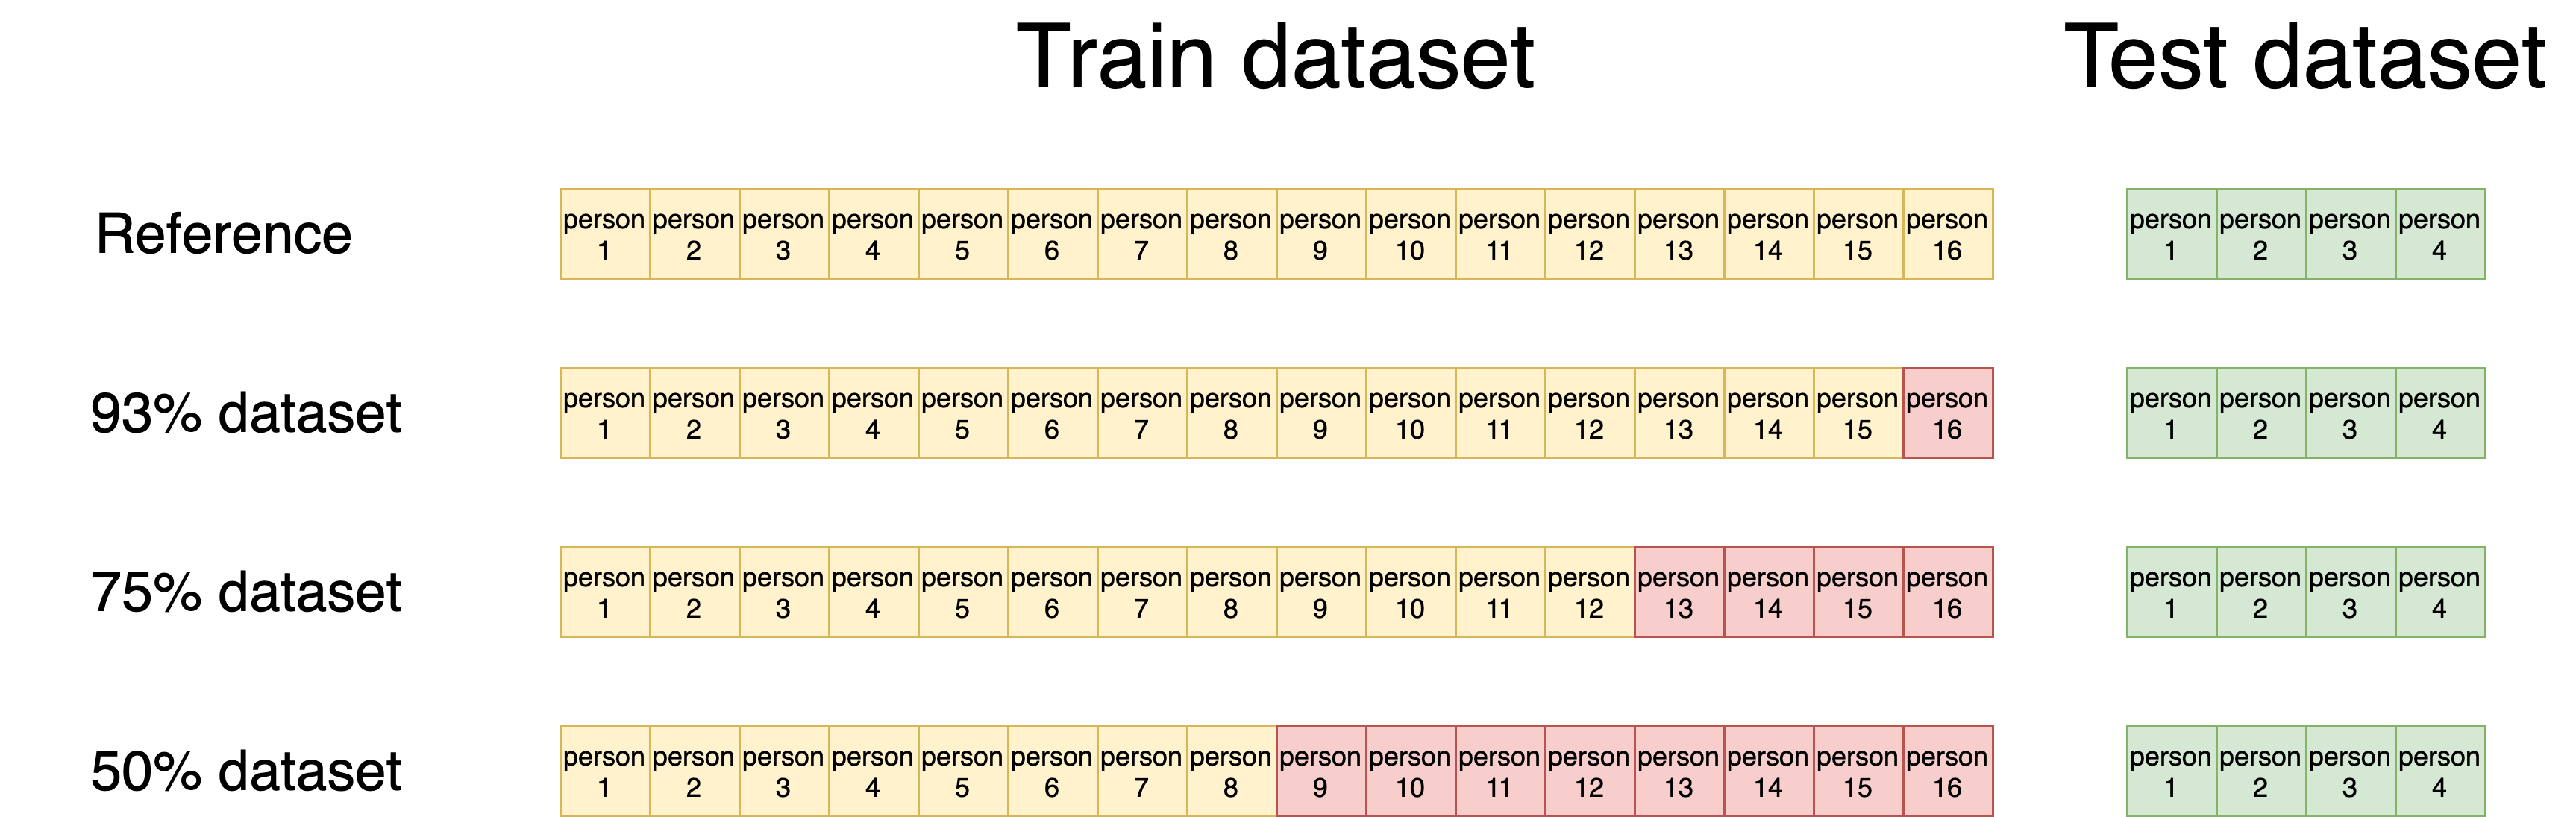
\includegraphics[scale=.13]{Figures/dataset-split.png}}
    \caption{Visualization of different dataset fractions. Each squad represent subset of point cloud for human model in dataset. Yellow - subset is used for training. Red - subset is not used for training. Green - test subsets}
    \label{img:dataset-split}
\end{figure}

